\documentclass[tikz, border=4pt]{standalone}
\usepackage{tikz}
\usepackage{tikz-timing}
\begin{document}
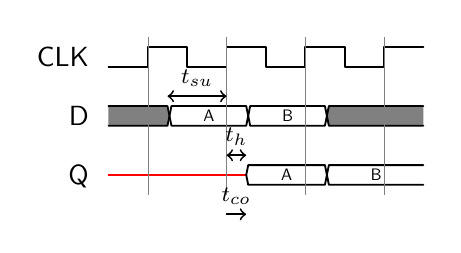
\begin{tikzpicture}[x=1cm, y=1cm]
  \node at (2.45,-1.13) {\pgfinterruptpicture%
  \begin{tikztimingtable}[timing/rowdist=3]
    CLK & 8{2C} \\
    D   & 3U 4D{A} 4D{B} 5U \\
    Q   & 7X 4D{A} 5D{B} \\
  \extracode
    \vertlines[help lines]{2,6,10,14}
    \draw [<->] (3,-1.5) -- node [above, font=\footnotesize] {$t_{su}$} (6,-1.5);
    \draw [<->] (6,-4.5) -- node [above, font=\footnotesize] {$t_{h}$} (7,-4.5);
    \draw [->] (6,-7.5) -- node [above, font=\footnotesize] {$t_{co}$} (7,-7.5);
  \end{tikztimingtable}%
  \endpgfinterruptpicture};
\end{tikzpicture}
\end{document}
